\documentclass[11pt]{article}

% load some asm stuff -
\usepackage{amssymb}
\usepackage{amsmath}
\usepackage{amsthm}
%\usepackage{palatino,lettrine}
\usepackage{fancyhdr}
\usepackage{epsfig}
\usepackage[square,sort,comma,numbers]{natbib}
\usepackage{simplemargins}
\usepackage{setspace}
\usepackage{wrapfig}
\usepackage{hyperref}
%\usepackage{boiboites}
\usepackage[margin=0pt,font=small,labelfont=bf]{caption}
\newcommand{\boldindex}[1]{\textbf{\hyperpage{#1}}}
\usepackage{makeidx}\makeindex
\bibliographystyle{plos2015}

\usepackage{algpseudocode}
\usepackage{algorithm}


% Set the size
%\textwidth = 6.75 in
%\textheight = 9.75 in
%\oddsidemargin = 0.0 in
%\evensidemargin = 0.0 in
%\topmargin = 0.01 in
%\headheight = 0.0 in
%\headsep = 0.25 in
%\parskip = 0.15in
% \doublespace
\setallmargins{1in}

\newtheorem{example}{Example}[section]
\newtheorem{thm}{Theorem}[section]
\newtheorem{property}{Property}[section]

\theoremstyle{definition}
\newtheorem{defn}[thm]{Definition}

\makeatletter
% \renewcommand\subsection{\@startsection
% 	{subsection}{2}{0mm}
% 	{-0.05in}
% 	{0.05\baselineskip}
% 	{\normalfont\normalsize\bfseries}}
\renewcommand\subsubsection{\@startsection
	{subsubsection}{2}{0mm}
	{-0.05in}
	{-0.5\baselineskip}
	{\normalfont\normalsize\itshape\bfseries}}
\renewcommand\paragraph{\@startsection
	{paragraph}{2}{0mm}
	{-0.05in}
	{-0.5\baselineskip}
	{\normalfont\normalsize\itshape}}
\makeatother
\linespread{1.1}

\fancypagestyle{proposal}{\fancyhf{}%
	\fancyhead[RO,LE]{\thepage}%
	\fancyhead[LO,RE]{CHEME 5660 Equity and Equity Prices}%
	\renewcommand\headrulewidth{1pt}}
\pagestyle{proposal}

\usepackage{mdframed}
\definecolor{lgray}{rgb}{0.92,0.92,0.92}
\definecolor{antiquewhite}{rgb}{0.98,0.92,0.84}
\definecolor{lightskyblue}{rgb}{0.93,0.95,0.99}

% defn environment
\mdfdefinestyle{theoremstyle}{% 
    linecolor=black,linewidth=1pt,% 
    frametitlerule=true,% 
    frametitlebackgroundcolor=lgray, 
    innertopmargin=\topskip,} 
\mdtheorem[style=theoremstyle]{definition}{Definition}

% concept environment
\mdfdefinestyle{conceptstyle}{% 
    linecolor=black,linewidth=1pt,% 
    frametitlerule=true,% 
    frametitlebackgroundcolor=lightskyblue, 
    innertopmargin=\topskip,} 
\mdtheorem[style=conceptstyle]{concept}{Concept}
\newcommand{\newterm}[1]{{\it #1}}

% Single space'd bib -
\setlength\bibsep{0pt}

\renewcommand{\rmdefault}{phv}\renewcommand{\sfdefault}{phv}
%\newboxedtheorem[boxcolor=black, background=gray!5,titlebackground=orange!20,titleboxcolor = black]{color_box_example}{Example}{test}

% Change the number format in the ref list -
\renewcommand{\bibnumfmt}[1]{#1.}

% Change Figure to Fig.
\renewcommand{\figurename}{Fig.}
\usepackage{enumitem}
\setlist{noitemsep} % or \setlist{noitemsep} to leave space around whole list

%Joycelyn Chan, Joshua Lequieu, Michael Paull, Chidanand Balaji, Ryan Tasseff
%Our derivation follows closely the earlier development of Fredrickson \citep{Fredrickson:1976fk}.

% Begin ...
\begin{document}

%\begin{titlepage}
{\par\centering\textbf{\Large Unit 2: Equity and Equity Pricing Models}}
\vspace{0.2in}
{\par \centering \large{Jeffrey D. Varner}}
\vspace{0.05in}
{\par \centering \large{Smith School of Chemical and Biomolecular Engineering}}
{\par \centering \large{Cornell University, Ithaca NY 14853}}
% \vspace{0.1in}
% {\par \centering \small{Copyright \copyright\ Jeffrey Varner 2018. All Rights Reserved.}}\\

%\end{titlepage}
\date{}
\thispagestyle{empty}

\setcounter{page}{1}

\section{Introduction}
In this unit, we will introduce the concept of equity and equity pricing models. 

\section{Lattice models of equity prices}
A lattice model discretizes the potential future states of the world into a finite number of options. 
For instance, a binomial lattice model has two future states: \texttt{up} and \texttt{down}, while a ternary lattice model has three: \texttt{up}, \texttt{down}, and \texttt{flat}. 
To make predictions, we must assign values and probabilities to each of these future states and then calculate the expected value and variance of future values. 
Thus, we do not precisely know quantities such as share price because we are projecting into the future. Instead, we have only a probabilistic model of the possible future values. 
We'll begin with the simplest possible lattice model, a binomial lattice (Fig. \ref{fig:binomial-lattice-schematic}).
\begin{figure}[h]
    \centering
    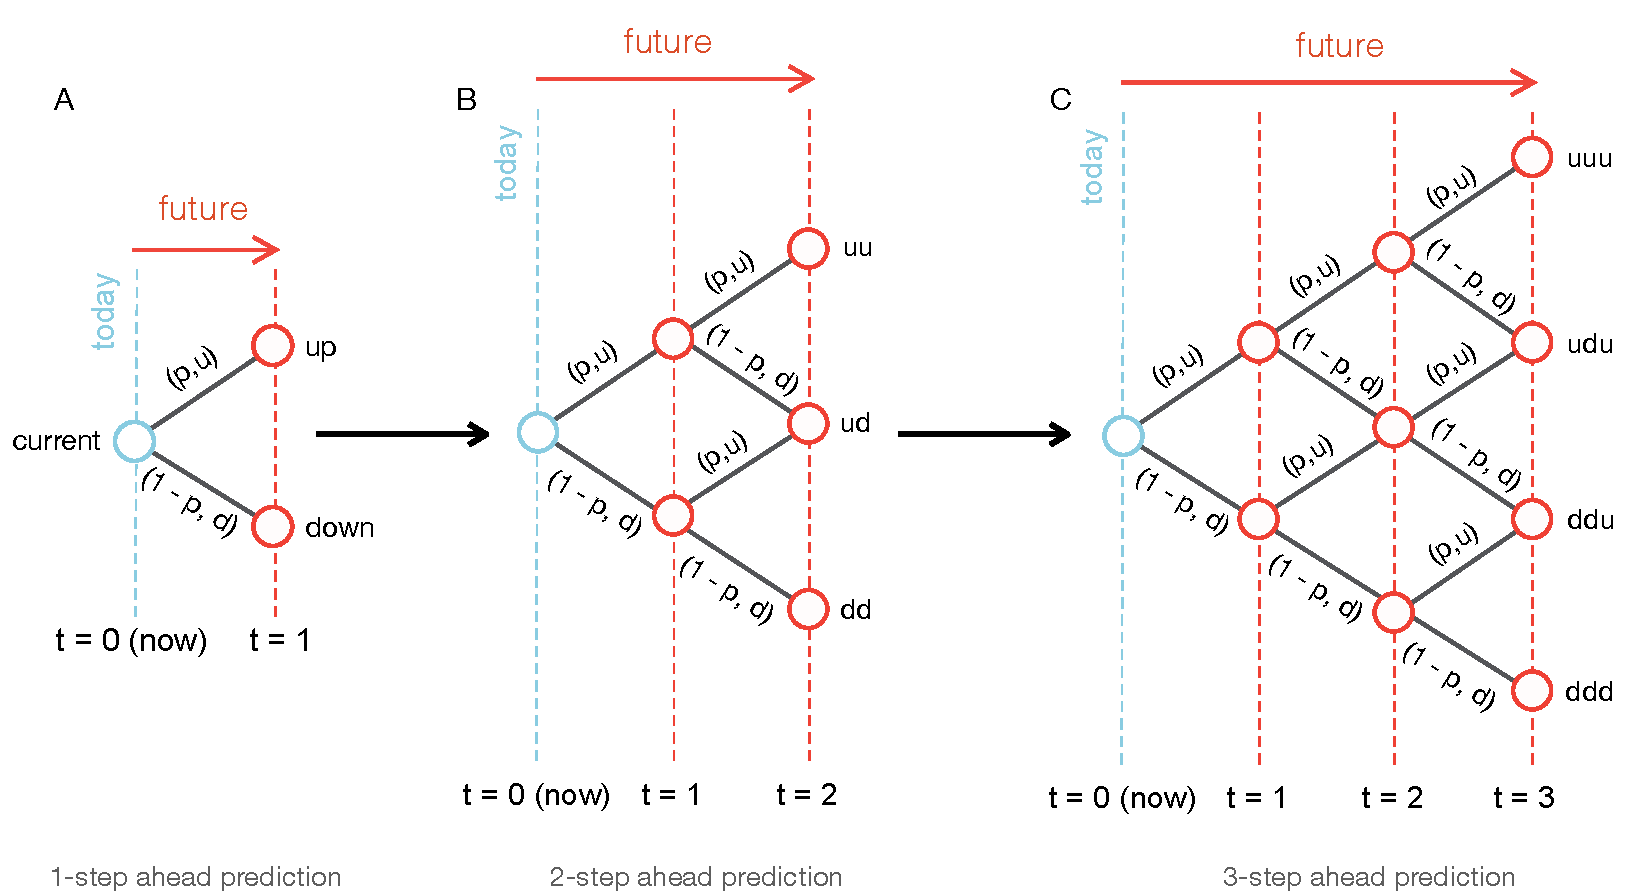
\includegraphics[width=0.85\textwidth]{./figs/Fig-Binomial-LatticeModels-Schematic.pdf}
    \caption{Binomial lattice model schematic. 
	At each node, the share price can either go \texttt{up} by $u$ or \texttt{down} by $d$. 
	The probability of going \texttt{up} is $p$, and the likelihood of going \texttt{down} is $1-p$. 
	\textbf{A}: Single time-step lookahead.
	\textbf{B}: Two time-step lookahead.
	\textbf{C}: Three time-step lookahead.
	At the tree $l$ level, the potential share price can take on $l+1$ values.
	}\label{fig:binomial-lattice-schematic}
\end{figure}

Let's start with a single time-step lookahead, with two possible future states (Fig. \ref{fig:binomial-lattice-schematic}A).
Let the initial share price at time \texttt{0} be $S_{\circ}$ and the share price at future time \texttt{1} be $S_{1}$.
During the transition from time \texttt{0}$\rightarrow$\texttt{1}, the world transitions from the current state to one of two possible future states: \texttt{up} or \texttt{down}.
We move to the \texttt{up} state with probability $p$ or the \texttt{down} state with probability $(1-p)$.
Thus, at the time \texttt{1}, the share price $S_{1}$ can take on one of two possible values: $S^{u} = u\cdot{S_{\circ}}$ if the world moves 
to the \texttt{up} state, or $S^{d} = d\cdot{S_{\circ}}$ if the world moves to the \texttt{down} state. 
As we move to the future, we can continue to build out the lattice model by adding additional time steps; for example, consider a two-step ahead prediction (Fig. \ref{fig:binomial-lattice-schematic}B). 
At time \texttt{2}, the share price can take on one of three possible values: $S^{uu} = u^{2}\cdot{S_{\circ}}$ if the world moves
to the \texttt{up-up} state, $S^{ud} = ud\cdot{S_{\circ}}$ if the world moves to the \texttt{up-down} state, or $S^{dd} = d^{2}\cdot{S_{\circ}}$ if the world moves to the \texttt{down-down} state.
We can continue to build out the lattice model by adding additional time steps; for example, consider a three-step ahead prediction (Fig. \ref{fig:binomial-lattice-schematic}C).

\subsection{Analytical solution}
Let's consider a binomial lattice model with $n$ time-steps. At each time step, the share price can either go \texttt{up} by a factor of $u$ or \texttt{down} by a factor of $d$.
Then, at time \texttt{n}, the share price can take on $n+1$ possible values: 
\begin{equation}
	S_{n} = S_{\circ}\times{D_{1}}\times{D_{2}}\times{D_{3}}\times\cdots\times{D_{n}}
\end{equation}
where $D_{i}$ is a random variable that can take on one of two values: $u$ or $d$, 
with probabilities $p$ and $(1-p)$ respectively. 
Thus, at each time-step, the world flips a coin and lands in either the \texttt{up} state with probability $p$ or the \texttt{down} state with probability $(1-p)$.
For a single time step, we model this random process as a Bernoulli trial, where the probability of success is $p$ and the likelihood of failure is $(1-p)$.
As the number of time steps increases, we have a series of Bernoulli trials, which is a binomial distribution (Defn: \ref{defn-binomial-distribution}):

\begin{definition}[Binomial Share Price and Probability]\label{defn-binomial-distribution}
	Let $S_{\circ}$ denote the current share price at t = \texttt{0}, $u$ and $d$ denote the \texttt{up} and \texttt{down} factors, 
	and $p$ denote the probability of going \texttt{up}.
	At time $t$, the binomial lattice model predicts the share price $S_{t}$ is given by:
	\begin{equation*}
	S_{t} = S_{\circ}\cdot{u}^{t-k}\cdot{d}^{k}\qquad\text{for}\quad{k=0,1,\dots,t}
	\end{equation*}
	The probability that the share price takes on a particular value at time $t$ is given by:
	\begin{equation*}
	P(S_{t} = S_{\circ}\cdot{u}^{t-k}\cdot{d}^{k}) = \binom{t}{k}\cdot{(1-p)}^{k}\cdot{p}^{t-k}\qquad\text{for}\quad{k=0,1,\dots,t}
	\end{equation*}
	where $\binom{t}{k}$ denotes the binomial coefficient.
\end{definition}

\subsection{Models of $u$, $d$ and $p$}
The \texttt{up} and \texttt{down} factors $u$ and $d$, and the probability $p$ can be computed in various ways.  
For example, we can estimate them from historical data or propose models for their values. 
Let's start by looking at approaches to estimate these parameters from historical data. Then, we'll introduce an important model developed by Cox, Ross, and Rubinstein (CRR) to compute $u$, $d$, and $p$ in the 
context of options pricing that we'll see later \citep{COX1979229}.

\subsubsection{Real-world probability $p$}
Suppose we have a historical share price dataset from time $1,\dots, T$ for some ticker $j$ denoted as $\mathcal{D}_{j} = \left\{S^{(j)}_{1}, S^{(j)}_{2},\dots, S^{(j)}_{T}\right\}$, 
where $S^{(j)}_{i}$ denotes the share price of ticker $j$ at time $i$.
We can use different values for the share price, e.g., the opening price, closing price, high price, low price, etc. 
When dealing with historical data, we will typically use the volume-weighted average price (VWAP) for the period, 
e.g., the VWAP for the day, week, month, etc. Over the time range of the dataset $\mathcal{D}_{j}$, we can calculate the number of \texttt{up} and \texttt{down} moves
occurring between time $i-1$ and $i$, and the magnitude of these moves. 
Then, the fraction of \texttt{up} moves is an estimate of the probability $p$, 
while some measured of the magnitude of the \texttt{up} and \texttt{down} moves, e.g., the average value are estimates of $u$ and $d$ respectively.

Suppose we assume the share price of ticker $j$ is continuously compounded with an instantaneous discount (interest) rate of 
$r^{(j)}_{i,i-1}\equiv\mu^{(j)}_{i,i-1}\cdot\Delta{t}$, i.e., we split the return into a growth rate $\mu^{(j)}_{i,i-1}$ and a time step size $\Delta{t}$.
Then, the share price at time an expression of the form governs $i$:
\begin{equation}\label{eqn:share-price-growth-rate}
S^{(j)}_{i} = \exp\left(\mu_{i,i-1}\cdot\Delta{t}\right)\cdot{S^{(i)}_{i-1}}
\end{equation}
where $\mu^{(j)}_{i,i-1}$ denotes the \textit{growth rate} (units: 1/time) for ticker $j$, and $\Delta{t}$ (units: time) 
is the time step size during the time period $(i-1)\rightarrow{i}$.
Solving for the growth rate (and dropping the ticker $j$ superscript for simplicity) gives:
\begin{equation}
\mu_{i,i-1} = \left(\frac{1}{\Delta{t}}\right)\cdot\ln\left(\frac{S_{i}}{S_{i-1}}\right)
\end{equation}
We often use daily price data; thus, a single trading day is a natural time frame between $S_{i-1}$ and $S_{i}$. 
However, subsequently, it will be easier to use an annualized value for the $\mu$ parameter; thus, we let $\Delta{t} = 1/252$, 
i.e., the fraction of an average trading year that occurs in a single trading day; thus, our base time will be years.
We compute the growth rate for each trading day $i$ in a collection of datasets $\mathcal{D}$ using Algorithm \ref{algo-log-return-distributions-equity}.
\begin{algorithm}[h]
    \caption{Logarithmic excess growth rate}\label{algo-log-return-distributions-equity}
    \begin{algorithmic}[1]
        
        \Require Collection of price datasets $\mathcal{D}$, where $\mathcal{D}_{j}\in\mathcal{D}$. All datasets have the same length $N$.	
		\Require list of stocks $\mathcal{L}$, where $\dim\mathcal{L} = M$.
        \Require time step size $\Delta{t}$ between $t$ and $t-1$ (units: years), 
        \Require risk-free rate $r_{f}$ (units: inverse years).

		\Statex
		\State{$M\leftarrow\text{length}(\mathcal{D}_{1})$}\Comment{Number of trading days in the dataset $\mathcal{D}_{j}$}
		\State{$N\leftarrow\text{length}(\mathcal{L})$}\Comment{Number of stocks in the dataset $\mathcal{D}$}
		\State{$\mu\leftarrow\text{Array}(M-1,N)$}\Comment{Initialize empty array of growth rates}
     
        \Statex
        \For{$i\in\mathcal{L}$}
			\State{$\mathcal{D}_{i} \gets \mathcal{D}[i]$}\Comment{Get dataset for stock $i$}

            \For{$t=2\rightarrow{N}$}
				\State{$S_{1} \gets \text{VWAP}(\mathcal{D}_{i}[t-1])$}\Comment{Get volume weighted average price for stock $i$ at time $t-1$}
				\State{$S_{2} \gets \text{VWAP}(\mathcal{D}_{i}[t])$}\Comment{Get volume weighted average price for stock $i$ at time $t$}
                
				\State{$\mu[t-1,i] \gets \left(\frac{1}{\Delta{t}}\right)\cdot\ln\left(\frac{S_{2}}{S_{1}}\right) - r_{f}$}\Comment{Set $r_{f} = 0$ for regular growth rate}
            \EndFor
        \EndFor
	
    \end{algorithmic}
\end{algorithm}
Then we can estimate the \texttt{up} and \texttt{down} factors $u$ and $d$ from the growth rate array 
generated using something like Algorithm \ref{algo-ud-estimation-equity}. 
\begin{algorithm}[h]
	\caption{Estimating $u$, $d$ and $p$ from the $\mu$-array}\label{algo-ud-estimation-equity}
	\begin{algorithmic}[1]

		\Require Growth-rate $\mu$-array from Algorithm \ref{algo-log-return-distributions-equity}.
		\Require Effective risk-free rate $\bar{r}$ (units: inverse years).
		\Require time step size $\Delta{t}$ between $t$ and $t-1$ (units: years) of the price data
		\Require \texttt{mean} function, \texttt{find} function, \texttt{length} function, and \texttt{push} function.

		\Statex
		\Procedure{real world probability}{$\mu$, $\bar{r}$, $\Delta{t}$}
		\State
		\State{\textit{Initialize}:}
		\State{$N\leftarrow\text{length}(\mu)$}\Comment{Number of growth rates}
		\State{$\text{up}\leftarrow\text{Array}()$}\Comment{Initialize empty array of \texttt{up} factors}
		\State{$\text{down}\leftarrow\text{Array}()$}\Comment{Initialize empty array of \texttt{down} factors}
		
		\Statex
		\State \textit{Compute $u$:}
   	 	\State{$i_{+}\leftarrow \text{find}(\mu>0)$}\Comment{Find the indices of all \texttt{positive} growth rates}
    	\For{$i\in {i_{+}}$}
			\State{$\text{push}(\text{up}, \exp(\mu[i]\cdot{\Delta{t}})))$}\Comment{Push the \texttt{positive} return $\mu\cdot\Delta{t}$ onto $\text{up}$-array}
    	\EndFor
		\State{$u\leftarrow\text{\texttt{mean}}(\texttt{up})$}\Comment{mean is our estimate of the \texttt{up} factor $u$}
    	
		\Statex
		\State \textit{Compute $d$:}
   	 	\State{$i_{-}\leftarrow \text{find}(\mu<0)$}\Comment{Find the indices of all \texttt{negative} growth rates}
    	\For{$i\in {i_{-}}$}
			\State{$\text{push}(\text{down}, \exp(\mu[i]\cdot{\Delta{t}}))$}\Comment{Push the \texttt{negative} return $\mu\cdot\Delta{t}$ onto $\text{down}$-array}
    	\EndFor
		\State{$d\leftarrow\text{\texttt{mean}}(\texttt{down})$}\Comment{mean is our estimate of the \texttt{down} factor $d$}



		\Statex
		\State{$N_{+} \leftarrow\text{length}(i_{+})$}\Comment{Number of \texttt{positive} growth rates}
		\State{$p\leftarrow N_{+}/N$}\Comment{Estimate of the probability $p$}
		\Statex

		\State
		\Return{$u$, $d$ and $p$}
		\Statex
		\EndProcedure
	\end{algorithmic}
\end{algorithm}
While this strategy is simple, it may not be robust. For example, if the dataset $\mathcal{D}_{j}$ is short, i.e., only a few trading days,
then the number of \texttt{up} and \texttt{down} moves will be small, and the estimates of $u$, $d$ and $p$ will be poor.
If a precise estimate of $u$, $d$ and $p$ is required, the number of trading days in the dataset $\mathcal{D}_{j}$ should be large.
Furthermore, the estimates of $u$, $d$ and $p$ are not robust to outliers in the dataset $\mathcal{D}_{j}$.
Thus, we may want to consider other models for computing $u$, $d$ and $p$.

\subsubsection{Risk-neutral probability $q$}
Another approach to computing the parameters in the lattrice is to use the risk-neutral probability $q$. 
Let's consider a single-step binomial lattice model (Fig. \ref{fig:binomial-lattice-schematic}A). 
The  expected value of the share price at time \texttt{1} for a single step is given by:
\begin{equation*}
	\mathbb{E}_{\mathbb{Q}}(S_{1} | S_{\circ}) = q\cdot{S^{u}} + (1-q)\cdot{S^{d}}
\end{equation*}
where $\mathbb{E}_{\mathbb{Q}}(\dots)$ denotes the expectation operator written with respect to the risk-neutral probability measure $\mathbb{Q}$, 
the term $q$ denotes the risk-neutral probability of the \texttt{up} state, and $S^{u}$ and $S^{d}$ are the share prices in the \texttt{up} and \texttt{down} states respectively.
The hypothetical probability $q$ is used to price derivatives (as we shall see later), 
however, we could also think of it as a tool to compute a \textit{fair} price for a share of stock.
Suppose we rewrite Eqn. \eqref{eqn:share-price-growth-rate} as:
\begin{equation}\label{eqn:share-price-growth-rate-2}
    \mathcal{D}_{1,0}(\bar{r})\cdot{S_{\circ}} = \mathbb{E}_{\mathbb{Q}}\left(S_{1}|S_{\circ}\right)
\end{equation}
where $\mathcal{D}_{1,0}(\bar{r})$ is the continuous discount factor between period $0\rightarrow{1}$, 
and $\bar{r}$ is the effective (constant) risk-free rate. Thus, unlike the previous case, where the share price $S_{i}$ was discounted by the
return $\mu_{i,i-1}\cdot\Delta{t}$ (which could vary in time), here we discount the share price $S_{i}$ by an effective (constant) risk-free rate $\bar{r}$.
The expectation operator $\mathbb{E}_{\mathbb{Q}}(\dots)$ can be matched with the expansion:
\begin{equation}\label{eqn:expectation-operator-risk-neutral}
\mathcal{D}_{1,0}(\bar{r})\cdot{S_{\circ}} = q\cdot{S^{u}} + (1-q)\cdot{S^{d}}
\end{equation}
The share prices in the \texttt{up} and \texttt{down} states are the product of the \texttt{up} factor $u$ (or a \texttt{down} factor $d$) and the initial share price, 
i.e., $S^{u} = u\cdot{S_{\circ}}$ and $S^{d} = d\cdot{S_{\circ}}$. Substiuting these price values into Eqn. \eqref{eqn:expectation-operator-risk-neutral} and solving for $q$ gives:
\begin{equation}\label{eqn:risk-neutral-probability}
q = \frac{\mathcal{D}_{1,0}(\bar{r}) - d}{u - d}
\end{equation}
Thus, we can compute the risk-neutral probability $q$ from the \texttt{up} and \texttt{down} factors $u$ and $d$ 
and the effective risk-free rate $\bar{r}$. The risk neutral probability $q$, and the \texttt{up} and \texttt{down} factors $u$ and $d$ 
can be estimated using Algorithm \ref{algo-risk-neutral-ud-estimation-equity}.

% \subsubsection*{Symmetric binomial lattice model.}
% The risk neutral probability $q$ is a function of the \texttt{up} and \texttt{down} factors $u$ and $d$ and the effective risk-free rate $\bar{r}$.
% Thus, we must still compute values (or propose models) for the \texttt{up} and \texttt{down} factors $u$ and $d$.
% One simple model is the symmetric binomial lattice model, where $u = 1/d$.

\begin{algorithm}[h]
	\caption{Risk-neutral estimate of $u$, $d$ and $q$}\label{algo-risk-neutral-ud-estimation-equity}
	\begin{algorithmic}[1]

		

		\Require Growth-rate $\mu$-array from Algorithm \ref{algo-log-return-distributions-equity}.
		\Require Effective risk-free rate $\bar{r}$ (units: inverse years).
		\Require time step size $\Delta{t}$ between $t$ and $t-1$ (units: years) of the price data
		\Require \texttt{mean} function, \texttt{find} function, \texttt{length} function, and \texttt{push} function.

		\Statex
		\Procedure{risk neutral probability}{$\mu$, $\bar{r}$, $\Delta{t}$}
		\State
		\State{\textit{Initialize}:}
		\State{$N\leftarrow\text{length}(\mu)$}\Comment{Number of growth rates}
		\State{$\text{up}\leftarrow\text{Array}()$}\Comment{Initialize empty array of \texttt{up} factors}
		\State{$\text{down}\leftarrow\text{Array}()$}\Comment{Initialize empty array of \texttt{down} factors}
		
		\Statex
		\State \textit{Compute $u$:}
   	 	\State{$i_{+}\leftarrow \text{find}(\mu>0)$}\Comment{Find the indices of all \texttt{positive} growth rates}
    	\For{$i\in {i_{+}}$}
			\State{$\text{push}(\text{up}, \exp(\mu[i]\cdot{\Delta{t}})))$}\Comment{Push the \texttt{positive} return $\mu\cdot\Delta{t}$ onto $\text{up}$-array}
    	\EndFor
		\State{$u\leftarrow\text{\texttt{mean}}(\texttt{up})$}\Comment{mean is our estimate of the \texttt{up} factor $u$}
    	
		\Statex
		\State \textit{Compute $d$:}
   	 	\State{$i_{-}\leftarrow \text{find}(\mu<0)$}\Comment{Find the indices of all \texttt{negative} growth rates}
    	\For{$i\in {i_{-}}$}
			\State{$\text{push}(\text{down}, \exp(\mu[i]\cdot{\Delta{t}}))$}\Comment{Push the \texttt{negative} return $\mu\cdot\Delta{t}$ onto $\text{down}$-array}
    	\EndFor
		\State{$d\leftarrow\text{\texttt{mean}}(\texttt{down})$}\Comment{mean is our estimate of the \texttt{down} factor $d$}

		\Statex
		\State{$q \gets \frac{\exp(\bar{r}\cdot{\Delta{t}}) - d}{u - d}$}\Comment{Compute the risk-neutral probability $q$}
		\Statex

		\State
		\Return{$u$, $d$ and $q$}
		\Statex
		\EndProcedure
	\end{algorithmic}
\end{algorithm}

\subsection{Cox-Ross-Rubinstein (CRR) model}
The \href{https://en.wikipedia.org/wiki/Binomial_options_pricing_model}{Cox, Ross, and Rubinstein (CRR) lattice model} 
assumes a risk-neutral probability $q$ to describe the probability of an \texttt{up} move. However, unlike a purely data-driven risk-neutral probability where we estimnate 
values for $u$ and $d$ from data, the CRR model proposes a model for $u$ and $d$ that is consistent with the variance of the return of the underlying asset.
The \texttt{up} factor $u$ is constructed so that the CRR model matches the variance of the log return $\text{Var}(S_{j}/S_{j-1})=\sigma^{2}\Delta{t}$:
\begin{equation*}
	\text{Var}(S_{j}/S_{j-1}) = \mathbb{E}\left[(S_{j}/S_{j-1})^{2}\right] - \mathbb{E}\left[S_{j}/S_{j-1}\right]^{2} = \sigma^{2}\Delta{t}
\end{equation*}
which after subtitution of the price and probability expressions from Defn. \ref{defn-binomial-distribution} gives:
\begin{equation}\label{eqn:variance-of-log-return}
    q(u-1)^{2} + (1-q)(d-1)^{2} + \left[p(u-1)+(1-q)(d-1)\right]^{2} = \sigma^{2}\Delta{t}
\end{equation}
where $\sigma$ is the volatility (standard deviation) of the return, and $\Delta{t}$ is the time step.
Equation \eqref{eqn:variance-of-log-return} is a quadratic equation in $u$, which can be solved for $u$ (assuming $\Delta{t}^{2}$ terms and above are ignored):
\begin{equation*}
    u = \exp(\sigma\cdot\sqrt{\Delta{t}})
\end{equation*} 
In the CRR approach, the \texttt{up} and \texttt{down} factors are related by $ud=1$, i.e., the lattice is symmetric.

To use the CRR model, we must first specify the volatility $\sigma$ of the return of the underlying asset, e.g., shares of stock.
We can estimate this from data by first computing the return (or the growth) and the estimatinf the volatility of the return, which is a backward-looking approach, 
or we can use the implied volatility from the options market, which is a forward-looking approach (the market's estimate of future price movements).

\subsection{Binomial lattice trade strategy}
Suppose we purchase $n_{o}$ share of ticker \texttt{XYZ} at time $t=0$ for $S_{o}$ USD/share.
Then, at some later date $t=T$, we sell all $n_{o}$ shares for $S_{T}$ USD/share. 
The net present value (NPV) of this trade has two cashflow events, the initial purchase of $n_{o}$ shares for $S_{o}$ USD/share,
and the sale of $n_{o}$ shares for $S_{T}$ USD/share at some later date $t=T$:
\begin{equation}
\text{NPV}(\bar{r},T) = -n_{o}\cdot{S_{o}} + n_{o}\cdot{S_{T}}\cdot\mathcal{D}_{T,0}^{-1}(\bar{r})
\end{equation}
where $\mathcal{D}_{T,0}^{-1}(\bar{r})$ is the inverse of the continuous discount factor 
for period $0\rightarrow{T}$, assuming an effective discount rate $\bar{r}$. 
Factoring the initial number of shares $n_{o}$ from the NPV expression gives:
\begin{equation}
\text{NPV}(\bar{r},T) = n_{o}\cdot\left(S_{T}\cdot\mathcal{D}_{T,0}^{-1}(\bar{r}) - S_{o}\right)
\end{equation}
The term in the parenthesis is the net change in the share price, i.e., the change in the share price $S_{T}$ discounted by the effective discount rate $\bar{r}$.
However, if we hold the shares for only a short period, e.g., on order days or months, then $\mathcal{D}_{T,0}^{-1}(\bar{r})\approx{1}$, which
simplifies the NPV expression to:
\begin{equation}
\text{NPV}(\bar{r}, T) \simeq n_{o}\cdot(S_{T}-S_{o})
\end{equation}
Dividing by the initial investment $n_{o}\cdot{S_{o}}$ gives the fraction return on investment, or just the fractional return:
\begin{equation}\label{eqn:roi-fractional-return}
\frac{\text{NPV}(\bar{r}, T)}{n_{o}\cdot{S_{o}}} \simeq \frac{S_{T}-S_{o}}{S_{o}} = \frac{S_{T}}{S_{o}} - 1
\end{equation}
In a binomial world, the share price $S_{T}$ is a random variable which takes on $T+1$ possible values:
\begin{equation}
S_{T} \in \left\{S_{\circ}\cdot{u}^{T-k}\cdot{d}^{k}\right\}_{k=0}^{T}
\end{equation}
where $S_{\circ}$ is the initial share price, $u$ and $d$ are the \texttt{up} and \texttt{down} factors, and $p$ is the probability of going \texttt{up}.
Substiuting the $S_{T}$ expression into Eqn. \eqref{eqn:roi-fractional-return} gives:
\begin{equation}\label{eqn:roi-fractional-return-2}
	\frac{\text{NPV}(\bar{r}, T)}{n_{o}\cdot{S_{o}}} \in \left\{u^{T-k}\cdot{d}^{k} - 1\right\}_{k=0}^{T}
\end{equation}
Equation \eqref{eqn:roi-fractional-return-2} describes the distribution of the fractional return on investment 
predicted by the binomial lattice model. Because we also have the probability of each future share price,
we can compute a number of interesting properties of the distribution of the fractional returns, e.g., the mean, variance, etc.
Furthermore, we can compute the probability that the fractional return is greater than some desired threshold, e.g., 10\%, by 
reconstructing the cumulative distribution function (CDF) of the fractional return.
We'll illustrate this idea with the project for this module.

\subsection{Summary}
In this module we introduced the binomial lattice model for equity share price. The binomial lattice model is a discrete-time model, 
where the furture share price can take on one of two possible values at each time step: \texttt{up} or \texttt{down}.
In the \texttt{up} state, the share price increases by a factor of $u$, while in the \texttt{down} state, the share price decreases by a factor of $d$.
The binomial lattice model is a probabilistic model, where the probability of going \texttt{up} is $p$ and the probability of going \texttt{down} is $(1-p)$.
The \texttt{up} and \texttt{down} factors $u$ and $d$, and the probability $p$ can be computed in various ways, but are assumed to be constant over time.
For example, we can compute the \texttt{up} and \texttt{down} factors $u$ and $d$ from historical data, or we can propose a model for $u$ and $d$.
Finally, we developed a simple trade strategy which relied on the binomial lattice model to compute a future price distribution, 
where the net present value was used to value the trade strategy.

\section{Single Asset Geometric Brownian Motion}
\href{https://en.wikipedia.org/wiki/Geometric_Brownian_motion}{Geometric Brownian motion (GBM)} is a continuous-time stochastic model in which the random variable $S(t)$, 
e.g., the share price of a firm. 
Geometric Brownian motion was popularized as a financial model by Samuelson in the 1950s and 1960s \cite{Merton2006}, 
but is arguably most commonly associated with the Black–Scholes options pricing model, which we will describe later 
\cite{BlackScholes1973}. Let's start with the single asset case (in the absence of dividends) 
and then consider the multiple asset case in the next module.

Geometric Brownian motion (GBM) assumes that the share price $S(t)$ of a firm can be modeled as a deterministic
drift term (which is proportional to the share price) that is corrupted by a \href{https://en.wikipedia.org/wiki/Wiener_process}{Wiener noise process}, also proportional to the share price:
\begin{equation}\label{eqn:GBM}
\frac{dS}{S} = {\mu}\,dt + \sigma\,{dW}
\end{equation}
The constant $\mu$ denotes a drift parameter, i.e., the growth rate of the share price return, $\sigma>0$ is a volatility parameter, i.e., 
the dispersion of the return, $dt$ denotes an infinitesimal time step, and $dW$ is the output of a 
\href{https://en.wikipedia.org/wiki/Wiener_process}{Wiener noise process}.  A \href{https://en.wikipedia.org/wiki/Wiener_process)}{Wiener Process} 
(also often referred to as a standard Brownian motion) is a real-valued continuous-time stochastic 
process named after \href{https://en.wikipedia.org/wiki/Norbert_Wiener}{Norbert Wiener} for the study of one-dimensional Brownian motion (Defn. \ref{defn-wiener-process}):
\begin{definition}[Wiener Process]\label{defn-wiener-process}
A Wiener process is a continuous one-dimensional stochastic process $\left\{W\left(t\right), 0\leq{t}\leq{T}\right\}$ with the following properties:
\begin{itemize}
\setlength\itemsep{0em}
\item{W$\left(0\right)$ = $0$ with probability $1$}
\item{The increments $\left\{W(t_{1}) - W(t_{o}),\dots, W(t_{k}) - W(t_{k-1})\right\}$ are independent for any $k$ and $0\leq{t_{o}}< t_{1} < \dots < t_{k} \leq{T}$}
\item{The increment W(t) - W(s) $\sim~N\left(0,t-s\right)$ for any $0\leq{s}< t \leq{T}$, where $N\left(0,t-s\right)$ denotes a normally distributed random variable with mean $0$ and variance $t - s$.}
\end{itemize}
\end{definition}
Equation \ref{eqn:GBM} is a continuous-time analog of the discrete-time binomial lattice model we developed previously. 
It has several exciting properties; for example, it has an analytical solution and analytical expressions for the expectation and variance of the share price. In this module, we will develop analytical solutions to Eqn. \ref{eqn:GBM}, and tools to estimate the parameters $\mu$ and $\sigma$ from historical data. We'll then use these tools to simulate the share price of firms and analyze properties of the return distributions in the example and project for this module. 

\subsection{Analytical solution}
Using Ito's lemma, we can formulate an analytical solution to the GBM equation for a single asset.
K. Ito's Lemma, developed in 1951, is an analog of the Taylor series for stochastic systems.
Let the random variable $X(t)$ be governed by the general stochastic differential equation:
\begin{equation*}
dX = a\left(X(t),t\right)dt + b\left(X(t),t\right)dW(t)
\end{equation*}
where $dW(t)$ is a one-dimensional Wiener process and $a$ and $b$ are functions of $X(t)$ and $t$. 
Let $Y(t) = \phi\left(t,X(t)\right)$ be twice differentiable with respect to $X(t)$, 
and singly differentiable with respect to $t$. Then, $Y(t)$ is governed by the equation:
\begin{equation*}
dY = \left(\frac{\partial{Y}}{\partial{t}}+a\frac{\partial{Y}}{\partial{X}}+\frac{b^{2}}{2}\frac{\partial^{2}{Y}}{\partial{X}^{2}}\right)dt+b\left(\frac{\partial{Y}}{\partial{X}}\right)dW(t)
\end{equation*}
Let $Y = \ln(S)$, $a = \mu\cdot{S}$, and $b = \sigma\cdot{S}$. 
Then, $Y$ is governed by the stochastic differential equation (using Ito's Lemma):
\begin{equation*}
d\ln(S) = \left(\mu - \frac{\sigma^{2}}{2}\right)dt + \sigma\cdot{dW(t)}
\end{equation*}
We integrate both sides of the equation to obtain from $t_{\circ}$ to $t$:
\begin{equation*}
\int_{t_{\circ}}^{t}d\ln(S) = \int_{t_{\circ}}^{t}\left(\mu - \frac{\sigma^{2}}{2}\right)dt + \int_{t_{\circ}}^{t}\sigma\cdot{dW(t)}
\end{equation*}
which gives:
\begin{equation*}
\ln\left(\frac{S_{t}}{S_{\circ}}\right) = \left(\mu - \frac{\sigma^{2}}{2}\right)\left(t - t_{\circ}\right) + \sigma\cdot\sqrt{t-t_{\circ}}\cdot{Z(0,1)}
\end{equation*}
where the noise term makes use of the definition of the integral of a Wiener process, and the properties of Normal random variables.
Finally, we exponentiate both sides of the equation to obtain the analytical solution to the GBM model:
\begin{equation}\label{eqn:analytical-soln-GBM}
S(t) = S_{\circ}\exp\Biggl[\left(\mu-\frac{\sigma^{2}}{2}\right)\left(t - t_{\circ}\right) + (\sigma\sqrt{t-t_{\circ}})\cdot{Z_{t}(0,1)}\Biggr]
\end{equation}
where $S_{\circ}$ denotes the share price at $t_{\circ}$, and $Z_{t}(0,1)$ denotes a 
\href{https://en.wikipedia.org/wiki/Normal_distribution#Standard_normal_distribution}{standard normal random variable} at time $t$.
The expectation and variance of the GBM model is given by:
\begin{eqnarray*}
\mathbb{E}\left(S_{t}\right) &=& S_{o}\cdot\exp\left(\mu\cdot\Delta{t}\right)\\
\text{Var}\left(S_{t}\right) &=& S_{\circ}^{2}e^{2\mu\cdot\Delta{t}}\left[e^{\sigma^{2}{\Delta{t}}} - 1\right]
\end{eqnarray*}
where $\Delta{t} = t - t_{\circ}$.

\subsection{Estimating the drift parameter $\mu$}
Let's assume that we have a time series of share price values $S(t_{1}), S(t_{2}), \dots, S(t_{k})$ and we want to estimate the detereministic growth of the share price, i.e., the drift parameter $\mu$.
There are several ways to do this, but we will use a detereministic linear model of the natural log of the share price values.
To estimate the deterministic component of the share price, we first set the volatility parameter $\sigma = 0$ in Eqn. \ref{eqn:analytical-soln-GBM}.
Then, at some future time $t$, the share price (after some algebra) is given by:
\begin{equation}\label{eqn:log-share-price-linear-model}
\ln\,S_{i} = \ln\,S_{\circ} + \mu\cdot\left(t_{i}-t_{\circ}\right)
\end{equation}
where $\ln\,S_{\star}$ denotes the natural log of the share price at time $t_{\star}$.
Equation \ref{eqn:log-share-price-linear-model} is a linear model of the form $y = mx + b$, where $y = \ln\,S_{i}$, $x = t_{i}-t_{\circ}$, $m = \mu$, and $b = \ln\,S_{\circ}$.
Thus, we can estimate the growth parameter $\mu$ by fitting a linear model to the log of the share price values by solving an overdetermined system of linear equations.

Let $\mathbf{A}$ denote a $\mathcal{S}\times{2}$ matrix, where each row corresponds to a time value $t>0$. 
The first column of $\mathbf{A}$ is all 1's while the second column holds the $(t_{k}-t_{\circ})$ values. 
Further, let $\mathbf{Y}$ denote the natural log of the share price values (in the same temperal order as the $\mathbf{A}$ matrix). 
Then, the y-intercept and slope (drift parameter) can be estimated by solving the overdetermined system of equations:
\begin{equation*}
\mathbf{A}\mathbf{\theta} + \mathbf{\epsilon} = \mathbf{Y}
\end{equation*}
where $\mathbf{\theta}$ denotes the vector of unknown parameters (the y-intercept and slope), and $\mathbf{\epsilon}$ denotes an error model, e.g., a normal distribution with mean zero and variance $\sigma_{\epsilon}^{2}$.
This system can be solved as:
\begin{equation*}
\mathbf{\theta} = (\mathbf{A}^{T}\mathbf{A})^{-1}\mathbf{A}^{T}\mathbf{Y} - (\mathbf{A}^{T}\mathbf{A})^{-1}\mathbf{A}^{T}\mathbf{\epsilon}
\end{equation*}
where $\mathbf{A}^{T}$ denotes the transpose of the matrix $\mathbf{A}$, and $(\mathbf{A}^{T}\mathbf{A})^{-1}$ denotes the inverse of the square matrix product $\mathbf{A}^{T}\mathbf{A}$. 
Finally, we can estimate the error term $\mathbf{\epsilon}$ by calculating the residuals:
\begin{equation*}
\mathbf{\epsilon} = \mathbf{Y} - \mathbf{A}\mathbf{\theta}
\end{equation*}
and then fitting a normal distribution to the residuals, using some technique such as maximum likelihood estimation, to compute the uncertainty in the estimate of the drift parameter $\hat{\mu}$ 
(where the $\hat{\star}$ denotes an estimate of the parameter).

\subsection{Estimating the volatility parameter $\sigma$}
Generally, methods to estimate the volatility parameter can be classified into two categories - historical volatility estimates based on past return data and future volatility 
estimates based on the \href{https://en.wikipedia.org/wiki/Implied_volatility}{Implied Volatility (IV)} of \href{https://en.wikipedia.org/wiki/Option_(finance)}{options contracts}. 
Here, we estimate the volatility $\sigma$ from historical data, i.e., from the past returns of the share price.
A return refers to the increase or decrease in the price of an asset, e.g., shares of a stock, over a specific period, e.g., minutes, days, weeks, or even years. 
Assume the share price of a stock at time $t$ is given by $S(t)$. Then, if we assume continuous compounding, the price of the stock at time $t+\Delta{t}$ is given by:
\begin{equation}
    S(t+\Delta{t}) = S(t)\cdot\exp\left(\mu\cdot{\Delta{t}}\right)
\end{equation}
where $\mu$ denotes the instantenous growth rate (units: inverse years) of the share price over the time horizon $t\rightarrow{t+\Delta{t}}$. 
The continuously compounded share price gives rise to the logarithmic return model (Defn. \ref{defn-log-return-1}):
\begin{definition}[Logarithmic Return]\label{defn-log-return-1}
Let $S_{i,t-1}$ denote the continuously compounding share price of ticker $i$ at time $t-1$. Then, at time $t$, the share price for ticker $i$, denoted as $S_{i,t}$,
is given by:
\begin{equation}
    S_{i,t} = S_{i,t-1}\cdot\exp\left(\mu^{(i)}_{t,t-1}\cdot{\Delta{t}}\right)
\end{equation}
where $\mu^{(i)}_{t,t-1}$ denotes the instantenous growth rate (units: inverse years) of ticker $i$ over time horizon $(t-1)\rightarrow{t}$, 
and $\Delta{t}$ is the time interval between $t-1$ and $t$ (units: years). The logarithmic return on asset $i$ over time horizon $(t-1)\rightarrow{t}$, 
denoted by $r^{(i)}_{t,t-1}$, is defined as:
\begin{equation}
r^{(i)}_{t,t-1} \equiv \ln\left(\frac{S_{i,t}}{S_{i,t-1}}\right) = \mu^{(i)}_{t,t-1}\cdot{\Delta{t}}
\end{equation} 
\end{definition}
Given Defn. \ref{defn-log-return-1}, we compute the logarithmic return distribution using Algorithm \ref{algo-log-return-distributions-equity}.
For each stock $i$, we compute the logarithmic return $\mu^{(i)}_{t,t-1}$ for each time interval $(t-1)\rightarrow{t}$, and then compute the mean and variance of the logarithmic return distribution.
\begin{algorithm}[h]
    \caption{Logarithmic Excess Growth Rate}\label{algo-log-return-distributions-equity}
    \begin{algorithmic}[1]

        \Statex
        \Require data set $\mathcal{D}_{i} = \left\{S_{i,t}\right\}_{t=1}^{N}\in\mathcal{D}$ where $S_{i,t}$ denotes the price of stock $i$ at time $t$, all stocks have the same time horizon $N\gg{2}$, 
		and $\mathcal{D}$ denotes the data set of all stocks.
        \Require The time interval $\Delta{t}$ between $t$ and $t-1$ (units: years), and a list of stocks $\mathcal{L} = \left\{i\right\}_{i=1}^{M}$ where $M = \dim\mathcal{L}$.
        \Require The risk-free rate $r_{f}$ (units: inverse years).
     
        \Statex
		\Procedure{log growth rate}{$\mathcal{D}$, $\mathcal{L}$, $\Delta{t}$, $r_{f}$}
		\State{$N\leftarrow\text{length}(\mathcal{D})$}\Comment{Number of trading days for each stock $i\in\mathcal{L}$}
        \For{$i\in\mathcal{L}$}
			\State{$\mathcal{D}_{i} \gets \mathcal{D}[i]$}\Comment{Select the data for stock $i$ from the dataset collection $\mathcal{D}$}
            \For{$t=2\rightarrow{N}$}
                \State{$S_{i,t-1} \gets \mathcal{D}_{i}[t-1]$}\Comment{Select the price of stock $i$ at time $t-1$}
                \State{$S_{i,t} \gets \mathcal{D}_{i}[t]$}\Comment{Select the price of stock $i$ at time $t$}
                \State{$\mu^{(i)}_{t,t-1} \gets \left(1/\Delta{t}\right)\cdot\ln\left(S_{i,t}/{S_{i,t-1}}\right) - r_{f}$}\Comment{Set $r_{f} = 0$ for regular growth rate}
            \EndFor
        \EndFor
        \Statex
        \Return{$\mu^{(1)},\dots,\mu^{(\dim\mathcal{L})}$}\Comment{Return the logarithmic growth rate array for each stock $i\in\mathcal{L}$}
		\EndProcedure
    \end{algorithmic}
\end{algorithm}
Once we estimated the logarithmic growth distribution for each stock, we can estimate the volatility parameter $\sigma$ by computing the standard deviation of the return distribution.
Typically, we use the daily data, but we want the annualized standard deviation of the logarithmic return distribution, thus we multiply the daily standard deviation by $\sqrt{252}$, where $252$ is the average number of trading days in a year, 
i.e, $\sigma\leftarrow \sqrt{252}\cdot\sigma$.

\subsection{Stylized facts}
Geometric Brownian motion is a widely used as a pricing model. 
However, whether geometric Brownian motion replicates many of the statistical properties of actual pricing and return data is unclear. 
These properties, referred to as \textit{stylized facts} have been observed for decades, 
dating back to early work of Mandelbrot \cite{Mandelbrot-1963,Mandelbrot-1967} and later by Cont \cite{Cont-QuantFinance-2001} 
and more recently by Ratliff-Crain et al. \cite{ratliffcrain2023revisiting} who reviewed the original stylized facts 
proposed by Cont using newer data.

Computing and understanding the stylized facts of financial data is important for several reasons. 
However, here we'll focus on only two, namely, the shape of the return distribution and the autocorrelation of the returns.
The shape of the return distribution is important because it is used to compute the probability of extreme events.
For example, the probability of a 10\% drop in the share price of a firm in a single day. 
Typiclly, we assume that the return distribution is normal, but this is not always the case. 
Instead, retruns are often leptokurtic, i.e., they have fat tails, for example following a Laplace distribution.
The autocorrelation of the returns is important because it is used to compute the probability of a run of consecutive up or down days.
If the returns are uncorrelated in time, then consecutive up or down days are independent events, i.e., 
the return (up or down) on day $t$ is independent of the return on day $t-1$. Thus, the market is behaving like a random walk.
However, if the returns are correlated in time, then consecutive up or down days are not independent events, i.e., 
past returns influence future returns. This is a very active area of research, and we will not be able to cover all of the stylized facts here. However, the 
the lack of autcorrelation goes to the heart of the efficient market hypothesis, which is at the core of modern finance theory, 
and one of the foundation principeles of quantitative finance over the last 50 years.

In the example and project for this module, we will compute the stylized facts of the share price of firms in the S\&P 500 index.
In particular, we will compute the shape of the return distribution and the autocorrelation of the returns. 
We'll show that the returns are leptokurtic, for the majority of the firms in the S\&P 500 index, and that the returns are uncorrelated in time.

\subsection{Summary}
In this module we introduced the single asset geometric Brownian motion model, and developed analytical solutions to the model.
This model is a continuous-time analog of the discrete-time binomial lattice model we developed previously.
The GBM model requires two parameters, the drift parameter $\mu$ and the volatility parameter $\sigma$. 
We developed methods to estimate these parameters from historical data, 
and then used these parameters to simulate the share price of firms in the example and project for this module.
Finally, we discussed the stylized facts of financial data, and particularly the shape of the return distribution and the autocorrelation of the returns.
The shape of the return distribution is important because it is used to compute the probability of extreme events, 
while the autcorrelation of the returns is important because it is used to compute the correlation in time of the returns. 

\section{Multiple Asset Geometric Brownian Motion Models}
\href{https://en.wikipedia.org/wiki/Geometric_Brownian_motion}{Geometric Brownian motion (GBM)} is a continuous-time stochastic model in which the random variable $S(t)$, 
e.g., the share price of a firm is described by a stochastic differential equation.
Geometric Brownian motion was popularized as a financial model by Samuelson in the 1950s and 1960s \cite{Merton2006}, 
but is arguably most commonly associated with the Black–Scholes options pricing model, which we will describe later 
\cite{BlackScholes1973}. Previously, we considered the single asset GBM model, 
where a firm's share price was modeled as a deterministic drift term corrupted by a Wiener noise process. 
We showed that a firm's share price follows a log-normal distribution and derived the analytical solution for a firm's share price at a future point in time.
However, in practice, investors often hold portfolios of assets, and a firm's share price is correlated with other firms' share price.
Thus, let's consider the GBM for multiple simultaneous assets, where the share price of a firm is modeled as a deterministic drift term 
that is corrupted by a Wiener noise process (same as before), but now we consider how the noise is correlated with other firms in a portfolio.

Consider an asset portfolio $\mathcal{P}$, e.g., a collection of equities with a logarithmic return covariance matrix $\Sigma$ and drift vector $\mu$.
The multi-dimensional geometric Brownian motion model describing the share price $S_{i}(t)$ for asset $i\in\mathcal{P}$ at time $t$ is given by: 
\begin{equation*}
\frac{dS_{i}\left(t\right)}{S_{i}(t)} = \mu_{i}\,{dt}+\sum_{j=1}^{\mathcal{P}}a_{ij}\cdot{dW_{j}(t)}\qquad\text{for}\quad{i=1,2,\dots,\mathcal{P}}
\end{equation*}
where $a_{ij}\in\mathbf{A}$ and $\mathbf{A}\mathbf{A}^{\top} = \Sigma$ are noise coefficients describing the connection between firms $i$ and firms $j$ in the portfolio $\mathcal{P}$,
and $\mu_{i}$ denotes the drift parameter for asset $i$ in the portfolio $\mathcal{P}$.
The multi-dimensional GBM model has the analytical solution:
\begin{equation*}
S_{i}(t_{k}) = S_{i}(t_{k-1})\cdot\exp\Biggl[\left(\mu_{i}-\frac{\sigma_{i}^{2}}{2}\right)\Delta{t} + \sqrt{\Delta{t}}\cdot\sum_{j\in\mathcal{P}}a_{ij}\cdot{Z_{j}(0,1)}\Biggr]\quad{i\in\mathcal{P}}
\end{equation*}
where $S_{i}(t_{k-1})$ is the share price for firm $i\in\mathcal{P}$ at time $t_{k-1}$,  the term $\Delta{t} = t_{k} - t_{k-1}$ denotes the time difference (step-size) 
for each time step (fixed), and $Z_{j}(0,1)$ is a standard normal random variable for firm $j\in\mathcal{P}$.
For more information on the derivation of the multi-dimensional GBM model, see Glasserman \cite{Glasserman:2004ua}.

\subsection{Drift and Covariance Estimation}
The drift vector $\mu$ and covariance matrix $\Sigma$ are critical parameters in the multi-dimensional GBM model.
We can estimate the drift vector $\mu$, which will be a $\dim\mathcal{P}\times{1}$ vector, from historical data by computing the logarithmic excess growth rate of the assets in the portfolio $\mathcal{P}$, 
as we have shown previously; we repeat the process for each asset in the portfolio $\mathcal{P}$.
On the other hand, the covariance matrix, a $\dim\mathcal{P}\times\dim\mathcal{P}$ symmetric matrix, describes the relationship between the logarithmic return series of firms $i$ and $j$.
The $(i,j)$ element of the covariance matrix $\sigma_{ij}\in\Sigma$ is given by:
\begin{equation*}
    \sigma_{ij} = \text{cov}\left(r_{i},r_{j}\right) = \sigma_{i}\sigma_{j}\rho_{ij}\qquad\text{for}\quad{i,j \in \mathcal{P}}
\end{equation*}
where $\sigma_{\star}$ denote the standard deviation of the logarithmic return of asset $\star$, i.e., the volatility parameter, and $\rho_{ij}$ 
denotes the correlation between the returns of asset $i$ and $j$ in the portfolio $\mathcal{P}$. 

The noise coefficients $a_{ij}$ modify the noise terms in the multi-dimensional GBM model, 
and describe the connection between firms $i$ and firms $j$ in the portfolio $\mathcal{P}$. 
The noise coefficients are given by the Cholesky decomposition of the covariance matrix $\Sigma$:
\begin{equation*}
\Sigma = \mathbf{A}\mathbf{A}^{\top}
\end{equation*}
where $\mathbf{A}$ is a lower triangular matrix, and $\mathbf{A}^{\top}$ denotes the complex conjugate transpose of $\mathbf{A}$. The diagonal elements of the Cholesky factor $\mathbf{A}$ are the standard deviations of the logarithmic return series of the assets in the portfolio $\mathcal{P}$, i.e., the volatility of firm $i$. On the other hand, the off-diagonal elements of the Cholesky factor $\mathbf{A}$ can be used to compute $\sigma_{ij}$, i.e., the covariance between the logarithmic return series of the assets in the portfolio $\mathcal{P}$. The Cholesky decomposition of the covariance matrix $\Sigma$ is unique and can be computed using the Cholesky decomposition algorithms provided by many common numerical linear algebra libraries.


\subsection{Multiasset Portfolio Simulations}
We simulate the multi-dimensional GBM model using the analytical solution for the share price of each firm in the portfolio $\mathcal{P}$, given the initial share price $\mathbf{S}(t_{0})$ vector, the drift vector $\mu$, the covariance matrix $\Sigma$, along with user-defined time points $t_{0},t_{1},\dots,t_{N}$, and the number of samples to simulate $N_{\text{samples}}$. 

\begin{definition}[Distribution of Share Price]\label{defn-log-normal-distribution-price}
The share price of each firm in the portfolio $\mathcal{P}$ at time $t$ follows a log-normal distribution:
\begin{equation*}
S(t)\sim\text{LogNormal}\left(\mu_{t},\Sigma_{t}\right)
\end{equation*}
where $\mu_{t}$ denotes the mean log-transformed share price vector, and $\Sigma_{t}$ denotes the covariance matrix of the log-transformed share prices at time $t$. A log-normal distribution is a right-skewed distribution. It is often used to model the share price because of its positive support and its ability to model the exponential growth of the share price.
\end{definition}
We simulate the multi-dimensional GBM model using Algorithm \ref{algo-multi-asset-gbm-simulation}, and then fit a distribution to the simulated share price of each firm in the portfolio $\mathcal{P}$ (Defn. \ref{defn-log-normal-distribution-price}).


\begin{algorithm}[h!]
    \caption{Multiasset Geometric Brownian Motion}\label{algo-multi-asset-gbm-simulation}
    \begin{algorithmic}[1]
		\Statex
		\Require The initial share price vector $\mathbf{S}(t_{0}) = \left\{S_{i}(t_{0})\right\}_{i=1}^{\dim\mathcal{P}}$ for each firm $i\in\mathcal{P}$.
		\Require The drift vector $\mu = \left\{\mu_{i}\right\}_{i=1}^{\dim\mathcal{P}}$ for each firm $i\in\mathcal{P}$.
		\Require The covariance matrix $\Sigma$ for the portfolio $\mathcal{P}$.
		\Require The time step $\Delta{t}$ (units: years), the initial time $t_{\circ}$, the final time $t_{f}$, and the number of samples $N_{s}$.
		\Require A Cholesky decomposition function $\texttt{cholesky}(\Sigma)$ that returns the Cholesky factor $\mathbf{A}$.

		\Statex
		\Procedure{Multiasset Geometric Brownian Motion}{}
		\Statex
		\State{$N_{a} \gets \text{length}(\mu)$}\Comment{Number of assets in the portfolio $\mathcal{P}$}
		\State{$N_{t} \gets (t_{f} - t_{\circ})/\Delta{t}$}\Comment{Number of time steps}
		\State{$T \gets \texttt{arange}(t_{\circ},t_{f},\Delta{t})$}\Comment{Time points}
		\State{$X \gets \texttt{zeros}(N_{s},N_{t}, N_{a}+1)$}\Comment{Pre-allocate the share price array}
		\State{$\mathcal{Z} \gets \mathcal{N}(0,1)$}\Comment{Instantiate a standard normal distribution}
		\State{$\mathbf{A} \gets \texttt{cholesky}(\Sigma)$}\Comment{Cholesky decomposition of the covariance matrix $\Sigma$}
		
		
		\Statex
		\For{$i\in{1}~\text{to}~{N_{s}}}$\Comment{Loop over the number of samples}
			
			\For{$j\in\texttt{eachindex}(T)$}\Comment{Loop over the time points}
				\State{$X_{i,j,1} \gets T_{j}$}\Comment{Set the time points in first column}
			\EndFor
			\Statex
			\For{$j\in{1}~\text{to}~N_{a}$}\Comment{Loop over the number of assets in the portfolio $\mathcal{P}$}
				\State{$X_{i,1,j+1} \gets S_{\circ,j}$}\Comment{Set the initial share price for asset $j$}
			\EndFor
			\Statex

			\For{$j\in{2}~\text{to}~N_{t}$}\Comment{Loop over the number of time steps}
				\For{$k\in{1}~\text{to}~N_{a}$}\Comment{Loop over the number of assets in the portfolio $\mathcal{P}$}
				\Statex
				\State{$\text{noise} \gets 0.0$}
				\For{$l\in{1}~\text{to}~N_{a}$}\Comment{Loop over the number of assets in the portfolio $\mathcal{P}$}
					\State{$\text{noise} \gets \text{noise} + \mathbf{A}_{k,l}\cdot\texttt{rand}(\mathcal{Z})$}\Comment{Compute the noise term for asset $k$}
				\EndFor
				\Statex
				\State{$X_{i,j,k+1} \gets X_{i,j-1,k+1}\cdot\exp\Biggl[\left(\mu_{k}-a_{kk}^2/{2}\right)\cdot\Delta{t} + \sqrt{\Delta{t}}\cdot\text{noise}\Biggr]$}
				\EndFor
			\EndFor
		\EndFor

		\EndProcedure
	\end{algorithmic}
\end{algorithm}

\subsection{Computing the Net Present Value (NPV) of a portfolio $\mathcal{P}$}
To compute the Net Present Value (NPV) of a portfolio $\mathcal{P}$, we can use Algorithm \ref{algo-multi-asset-gbm-simulation} to simulate the share price of each firm in $\mathcal{P}$ over a time-horizon, e.g., from now to until next year.
Given the share price of each firm over that horizon, we can compute what combinations of shares of each firm in the portfolio $\mathcal{P}$ are the best in some way. For example, we can compute which share combinations lead to the largest projected NPV of the portfolio $\mathcal{P}$ at time $t$ by computing the 
two cash flow events that occur, first the purchase of the shares of each firm in the portfolio $\mathcal{P}$ at time $t_{0}$, and then the liquidation of the portfolio $\mathcal{P}$ at time $T$, where the future share price value is discounted back to the present value using an appropriate discount rate, such as the average risk-free rate over the period $\bar{r}_{f}$:
\begin{equation}\label{eqn:npv-mv-gbm}
\text{NPV}(T,\bar{r}_{f}) = \sum_{i\in\mathcal{P}}n_{i}\cdot\left(\mathcal{D}_{T,0}^{-1}(\bar{r}_{f})\cdot{S_{i}(T)}-S_{i}(0)\right)
\end{equation}
where $n_{i}$ denotes the number of shares of firm $i\in\mathcal{P}$, $S_{i}(T)$ denotes the share price of firm $i\in\mathcal{P}$ at time $T$, $S_{i}(0)$ denotes the share price of firm $i\in\mathcal{P}$ at time $0$, and $\mathcal{D}_{T,0}(\bar{r}_{f})$ denotes the multiperiod discount factor between time $0\rightarrow{T}$ with the discount rate equal to the risk-free rate $\bar{r}_{f}$.

To calculate the net present value at $t=T$, we need the share price of each firm in the portfolio $\mathcal{P}$ at time $T$ and the number of shares of each firm in the portfolio $\mathcal{P}$ at time $t_{0}$, 
where we assume the investor does not buy or sell any shares of any firm in the portfolio $\mathcal{P}$ over the period $t_{0}\rightarrow{T}$. The number of shares of each firm in the portfolio $\mathcal{P}$ at time $t$ is given by the fraction of the total wealth invested in each firm in the portfolio $\mathcal{P}$. Let's imagine a scenario where an investor has a total wealth of $W_{\text{total}}$ at time $t$, and the fraction of the total wealth invested in each firm $i\in\mathcal{P}$ is given by $0\leq{\omega_{i}}\leq{1}$:
\begin{equation*}
\omega_{i}(t) = \frac{W_{i}(t)}{W_{\text{total}}}\qquad\text{for}\quad{i\in\mathcal{P}}
\end{equation*}
where $W_{i}(t)$ denotes the wealth invested in firm $i\in\mathcal{P}$ at time $t$.
However, we know the total wealth of portfolio $\mathcal{P}$, is just the liqidation value of the portfolio: 
\begin{equation*}
W(t) = \sum_{i\in\mathcal{P}}n_{i}(t)\cdot{S_{i}(t)}
\end{equation*}
where $n_{i}(t)$ denotes the number of shares of firm $i\in\mathcal{P}$ at time $t$, and $S_{i}(t)$ denotes the share price of firm $i\in\mathcal{P}$ at time $t$. We can rewrite the number of shares of each firm in the portfolio $\mathcal{P}$ at time $t$ as:
\begin{equation*}
	n_{i}(t) = \frac{\omega_{i}(t)\cdot{W_{\text{total}}}}{S_{i}(t)}\qquad\text{for}\quad{i\in\mathcal{P}}
\end{equation*}
Further, we can rewrite the fraction of the total wealth invested in each firm $i\in\mathcal{P}$ as:
\begin{equation}\label{eqn:portfolio-weights-derivation}
\omega_{i}(t) = \frac{n_{i}(t)\cdot{S_{i}(t)}}{\displaystyle\sum_{k\in\mathcal{P}}n_{k}(t)\cdot{S}_{k}(t)}\qquad\text{for}\quad{i\in\mathcal{P}}
\end{equation}
The fractions $\omega_{i}(t)$, i.e., the portfolio weights at time $t$, have a few interesting properties (Concept \ref{concept:properties-of-omega}).

\begin{concept}[Properties of allocation $\omega$]\label{concept:properties-of-omega}
The fraction of the total wealth invested in each firm $i\in\mathcal{P}$ at time $t$, in the absence of borrowing shares, sums to one for all time points $t$:
\begin{equation*}
\sum_{i\in\mathcal{P}}\omega_{i}(t) = 1\quad\forall{t\geq{t_{0}}}
\end{equation*}
Further, because the share price of each firm in the portfolio $\mathcal{P}$ is positive, the fraction of the total wealth invested in each firm $i\in\mathcal{P}$ at time $t$ is non-negative $\omega_{i}(t)\geq{0}$ for all $t\geq{t_{0}}$. 
Finally, $\omega_{i}$, even with constant shares, is a function of time as the share price of each firm in the portfolio $\mathcal{P}$ changes over time.
\end{concept}
The investor can choose the fraction of the total wealth $\omega_{i}$ invested in each firm $i\in\mathcal{P}$ by some approach, e.g., by formulating the choice as an optimization problem or by sampling from a probability distribution such as a Dirchlet distribution $\omega_{i}\sim\text{Dirchlet}(\alpha_{1},\alpha_{2},\dots,\alpha_{\dim\mathcal{P}})$, where $\alpha_{i}$ denotes the concentration parameter for firm $i\in\mathcal{P}$. Then, when combined with the multi-dimensional GBM model, the investor can simulate the share price of each firm in the portfolio $\mathcal{P}$ over a time period and compute the NPV of the portfolio. This process can be repeated many times, and the expected NPV of the portfolio $\mathcal{P}$ at time $T$ can be computed by averaging the NPV over all the samples (Algorithm \ref{algo-npv-monte-carlo-portfolios}).

\begin{algorithm}[h]
	\caption{Monte-Carlo Portfolio Net Present Value}\label{algo-npv-monte-carlo-portfolios}
	\begin{algorithmic}[1]
		\Require The initial share price vector $\mathbf{S}(t_{0}) = \left\{S_{i}(t_{0})\right\}_{i=1}^{\dim\mathcal{P}}$ for each firm $i\in\mathcal{P}$.
		\Require Share price distribution $S(T)\sim\text{LogNormal}(\mu_{T},\Sigma_{T})$ 
		\Require An allocation distribution function $\omega\sim\text{Dir}(\alpha_{1},\alpha_{2},\dots,\alpha_{\dim\mathcal{P}})$, where we assume equal concentration parameters $\alpha_{i}=1/\dim\mathcal{P}$ firm $i\in\mathcal{P}$.
		\Require The average risk-free rate $\bar{r}_{f}$, the number of samples $N_{s}$ and the total wealth $W_{\text{total}}$.
		\Statex
		\Procedure{Portfolio Simulation}{}
		\Statex
		\State{$\text{NPV} \gets \texttt{zeros}(N_{s}, \dim\mathcal{P}+1)$}\Comment{Pre-allocate the NPV array}
		\For{$i\in{1}~\text{to}~N_{s}$}\Comment{Loop over the number of samples}
			\State{$\mathbf{S} \gets S(T)$}\Comment{Sample the share price of each firm in the portfolio $\mathcal{P}$ at time $T$}
			\State{$\omega \gets \text{Dir}(\alpha)$}\Comment{Sample allocation $\omega$ at $t=t_{0}$}
			\Statex
			\State{$n\gets \texttt{zeros}(\dim\mathcal{P})$}\Comment{Pre-allocate the number of shares array}
			\For{$j\in{1}~\text{to}~\dim\mathcal{P}$}\Comment{Loop over the number of assets in the portfolio $\mathcal{P}$}
				\State{$n_{j}\gets \omega_{j}\cdot{W}_{\text{total}}\cdot\left(S_{j}(t_{0})^{-1}\right)$}\Comment{Compute the number of shares of firm $j$ at time $t = t_{0}$}
			\EndFor
			\Statex
			\State{$\text{NPV}_{i,1} \gets \sum_{k\in\mathcal{P}}n_{k}\cdot\left(\mathcal{D}_{T,0}^{-1}(\bar{r}_{f})\cdot{S_{k}(T)}-S_{k}(0)\right)$}\Comment{NPV of $\mathcal{P}$ at $T$, store column 1}

			\For{$j\in{1}~\text{to}~\dim\mathcal{P}$}\Comment{Loop over the number of assets in the portfolio $\mathcal{P}$}
				\State{$\text{NPV}_{i,j+1} \gets \omega_{j}$}\Comment{Store the portfolio weights in columns $2,\dots,\dim\mathcal{P}+1$}
			\EndFor

		\EndFor
		\Statex
		\EndProcedure

	\end{algorithmic}
\end{algorithm}

\subsection{Summary}
In this module, we have considered the multi-dimensional GBM model, 
which describes the share price of firms in a portfolio $\mathcal{P}$.
We demonstrated how to estimate the drift vector $\mu$, the covariance matrix $\Sigma$, and the noise coefficients $a_{ij}$, and provided an algorithm to simulate the multi-dimensional GBM model. Finally, we introduced the concept of the Net Present Value (NPV) of a portfolio $\mathcal{P}$. We presented an algorithm to compute the NPV of a portfolio $\mathcal{P}$ at time $T$, 
where we sampled the fraction of the total wealth $\omega_{i}$ invested in each firm $i\in\mathcal{P}$ from a Dirichlet distribution and the share price at $t=T$ from a LogNormal distribution. Later, we'll develop tools to compute optimal values of these fractions, i.e., the portfolio weights, but for now, we considered the case where the portfolio weights are chosen by the investor by some approach (perhaps even randomly).

\bibliography{References_v1}

\clearpage
\printindex

\end{document}
